\documentclass[onecolumn]{article}
\usepackage{graphicx}
\usepackage{float}
\usepackage{hyperref}
\restylefloat{figure}
\begin{document}

\title{Intersecting cubes and spheres}

\author{Arjen Markus}

\maketitle

\section*{Introduction}
This note is about the volumes of included and excluded bits and pieces of cubes and spheres that intersect.
As far as I know there is nothing practical about it, it just happened to attract my attention.

To define the problem: consider a cube and a sphere with different sizes but having the same centre.
Parts of the cube or parts of the sphere may stick out and the question is how large is the volume
of these parts? The answer depends on the relative size of the two and in some cases it will be
awkward to calculate.

Figure \ref{square_circle} is an illustration in two dimensions of the problem:

\begin{figure}[H]
\caption{Intersection of a square (side 2) and a circle: (A) circle with radius 1, (B) circle with radius $\sqrt{2}$}.
\label{square_circle}
\begin{center}
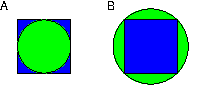
\includegraphics[width=0.7\textwidth]{circle_square_sketch.pdf}
\end{center}
\end{figure}

In the left half of the figure (A), the square is larger than the circle and it is easy to calculate
the area that lies outside the circle:
\begin{eqnarray}
\nonumber    A &=& 2^2 - \pi \cdot 1^2 \\
\nonumber      &=& 4 - \pi \\
\nonumber      &\approx& 0.8584073464102069
\end{eqnarray}

In the right half (B), the circle touches the vertices of the square and the area of the circle
outside the square is:
\begin{eqnarray}
\nonumber    A &=& \pi \cdot (\sqrt{2})^2 - 2^2 \\
\nonumber      &=& 2\pi - 4 \\
\nonumber      &\approx& 2.2831853071795862
\end{eqnarray}

\begin{figure}[H]
\caption{Rough sketch of a sphere touching the edges of the cube.}
\label{sphere_cube}
\begin{center}
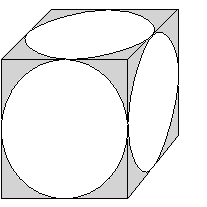
\includegraphics[width=0.5\textwidth]{sphere_cube_sketch.pdf}
\end{center}
\end{figure}

It is actually easy to calculate these areas for any radius of the circle.

\section*{The three-dimensional case}
For the intersection of a cube and a sphere we have three more or less special situations:
\begin{itemize}
\item
The sphere touches the centres of the cube's faces -- the radius is equal to half the side of the cube.
It is akin to figure \ref{square_circle}A. The volume outside the sphere is:
\begin{eqnarray}
\nonumber    V &=& 8 - \frac{4}{3} \pi \cdot 1^3 ~\approx~ 3.8112097952136095
\end{eqnarray}

\item
The sphere touches the vertices of the cube -- the radius is equal to $\sqrt{3}$ times the side of the cube.
This is akin to figure \ref{square_circle}B. The volume outside the cube is:
\begin{eqnarray}
\nonumber    V &=& \frac{4}{3} \pi \cdot (\sqrt{3})^3 - 8 ~\approx~ 13.765592370810609
\end{eqnarray}
\item
The sphere touches the midpoints of the edges of the cube -- the radius is equal to $\sqrt{2}$ times the side of the cube.
This has no easy equivalent to the two-dimensional case and calculating the volumes is a bit more involved, but not
overly difficult. (Radii between $\sqrt{2}$ and $\sqrt{3}$ create much more difficulties and are not included here.)
\end{itemize}

\begin{figure}[H]
\caption{Sketch of the spherical cap. The radius of the sphere $R = \sqrt{2}$.}
\label{integral}
\begin{center}
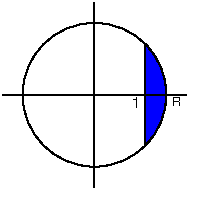
\includegraphics[width=0.5\textwidth]{integral_chord.pdf}
\end{center}
\end{figure}

This last case requires some ingenuity:
\begin{itemize}
\item
We first need to determine how much of the sphere sticks out. As illustrated in Figure \ref{sphere_cube} the
parts that stick out are spherical caps. The volume is easy to calculate (see Figure \ref{integral}):
\begin{eqnarray}
\nonumber V_{cap} &=& \int_{1}^{\sqrt{2}} \pi (2 - x^2) dx \\
\nonumber         &=& \left [2 \pi x - \frac{1}{3} \pi x^3 \right ]_{1}^{\sqrt{2}} \\
\nonumber         &=& \frac{4}{3} \pi \sqrt{2} - \frac{5}{3} \pi \\
\nonumber         &\approx& 0.6878561615614993
\end{eqnarray}

\item
As there are six such caps, the total volume of the sphere outside the cube is $8 \pi \sqrt{2} - 10 \pi$. This
needs to be subtracted from the total volume of the sphere itself to get the volume included in the cube.

\item
The volume of the cube outside the intersection with the sphere is therefore:
\begin{eqnarray}
\nonumber V &=& 8 - \left ( \frac{4}{3} \pi (\sqrt{2})^3 - (8 \sqrt{2} - 10) \pi \right ) \\
\nonumber   &=& 8 + \frac{16}{3} \pi \sqrt{2} - 10 \pi \\
\nonumber   &\approx& 0.2794491342800214
\end{eqnarray}

\end{itemize}

As said, for the situation that the sphere's radius is between $\sqrt{2}$ and $\sqrt{3}$, this method
does not work. The caps would partially overlap and you need to compensate for that to get the right
answer. A brute-force method would be to determine the volume of the corners directly, but this leads
to complicated three-dimensional integrals.

\end{document}

